% ------------------------------------------------------------------------------
% TYPO3 CMS 6.2 LTS - What's New - Chapter "Install Tool" (Italian Version)
%
% @author Roberto Torresani <roberto.torresani@typo3.org>
% @license	Creative Commons BY-NC-SA 3.0
% @link		http://typo3.org/download/release-notes/whats-new/
% @language	Italian
% ------------------------------------------------------------------------------
% Chapter: Install Tool
% ------------------------------------------------------------------------------

\section{Strumento di installazione}
\begin{frame}[fragile]
	\frametitle{Strumento di installazione}

	\begin{center}\huge{Capitolo 1:}\end{center}
	\begin{center}\huge{\color{typo3darkgrey}\textbf{Lo Strumento di installazione}}\end{center}

\end{frame}

% ------------------------------------------------------------------------------
% Installation
% ------------------------------------------------------------------------------

\begin{frame}[fragile]
	\frametitle{Strumento di installazione}
	\framesubtitle{Installazione}

	\begin{itemize}
		\item Solo \underline{un} pacchetto è richiesto per l'installazione:\newline
				\texttt{typo3\_src-6.2.x.tar.gz} (dimensione file: circa 20MB)
		\item I pacchetti "Dummy" e "Blank" diventano obsoleti
		\item Installazione:
			\begin{itemize}
				\item Estrai il pacchetto sorgente nella directory web principale
				\item Crea i link simbolici come richiesto
				\item Apri il browser web sulla pagina principale
				\item L'installazione TYPO3 inizia con i passi guidati '1-2-3-4'
			\end{itemize}

	\end{itemize}

\end{frame}

% ------------------------------------------------------------------------------
% Installation
% ------------------------------------------------------------------------------

\begin{frame}[fragile]
	% \TabPositions{2cm}

	\frametitle{Strumento di installazione}
	\framesubtitle{Installazione}

	\begin{itemize}
		\item Il processo di installazione verifica che tutte le directory e i file necessari siano corretti
		\item I file necessari per una configurazione personalizzata saranno creati automaticamente
		\item I seguenti link simbolici \underline{devono} essere presenti:

		\begin{itemize}
			\item \texttt{typo3\_src}	\tabto{2cm} (punta alla directory sorgente di TYPO3)
			\item \texttt{typo3}		\tabto{2cm} (punta alla directory: \texttt{typo3\_src/typo3})
			\item \texttt{index.php}	\tabto{2cm} (punta al file: \texttt{typo3\_src/index.php})
		\end{itemize}

		\item Nessun altro file/directory sono necessari per l'installazione di TYPO3!
		\item La directory \texttt{t3lib} è stata rimossa
		\item Altre indicazioni: TYPO3 Installation and Upgrade Guide\newline
			\url{http://docs.typo3.org/typo3cms/InstallationGuide}

	\end{itemize}

\end{frame}

% ------------------------------------------------------------------------------
% Re-Development
% ------------------------------------------------------------------------------

\begin{frame}[fragile]
	\frametitle{Strumento di installazione}
	\framesubtitle{Risviluppo}

	\begin{columns}[T]

		\begin{column}{.5\textwidth}
			\begin{itemize}
				\item Risviluppo da zero utilizzando Fluid
				\item Il \underline{primo} passo verifica l'ambiente di sistema e riporta eventuali problemi
				\item Le segnalazioni possono essere corrette (e riverificate) o ignorate
				\item Le configurazioni di base errate (es: mancanza dei link simbolici) sono segnalate
			\end{itemize}
		\end{column}

		\begin{column}{.5\textwidth}
			\begin{figure}\vspace*{-0.4cm}
				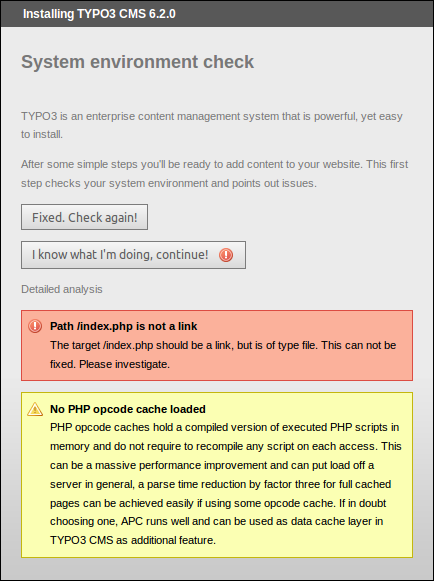
\includegraphics[width=0.8\linewidth]{Images/InstallTool/SystemEnvironmentCheck.png}
			\end{figure}
		\end{column}

	\end{columns}

\end{frame}

% ------------------------------------------------------------------------------
% Re-Development
% ------------------------------------------------------------------------------

\begin{frame}[fragile]
	\frametitle{Strumento di installazione}
	\framesubtitle{Risviluppo}

	\begin{columns}[T]

		\begin{column}{.5\textwidth}
			\begin{itemize}
				\item Il \underline{secondo} passo permette agli utenti di inserire le credenziali di accesso al database
				\item Il tipo di connessione è selezionabile
					\begin{itemize}
						\item Connessione basata su TCP/IP
						\item Connessione basata su socket
					\end{itemize}
				\item Sono possibili alternative a MySQL
			\end{itemize}
		\end{column}

		\begin{column}{.5\textwidth}
			\begin{figure}\vspace*{-0.4cm}
				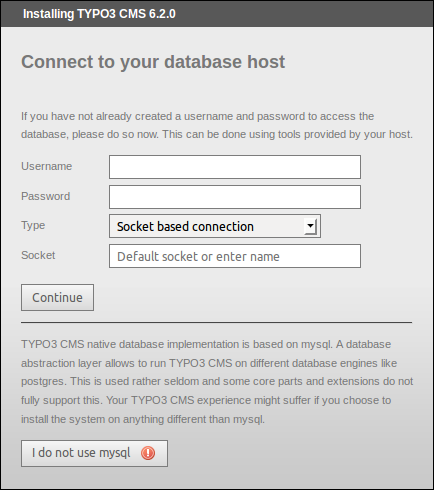
\includegraphics[width=0.8\linewidth]{Images/InstallTool/DatabaseConnectionDetails.png}
			\end{figure}
		\end{column}

	\end{columns}

\end{frame}

% ------------------------------------------------------------------------------
% Re-Development
% ------------------------------------------------------------------------------

\begin{frame}[fragile]
	\frametitle{Strumento di installazione}
	\framesubtitle{Risviluppo}

	\begin{columns}[T]

		\begin{column}{.5\textwidth}
			\begin{itemize}
				\item Il \underline{terzo} passo permette agli utenti di selezionare/creare il database\newline
					(come in TYPO3 < 6.2)
				\item Il \underline{quarto} passo permette agli utenti di impostare la password per l'utente "admin"\newline (che è anche la password iniziale dello strumento di installazione) e il nome del sito
			\end{itemize}
		\end{column}

		\begin{column}{.5\textwidth}
			\begin{figure}\vspace*{-0.4cm}
				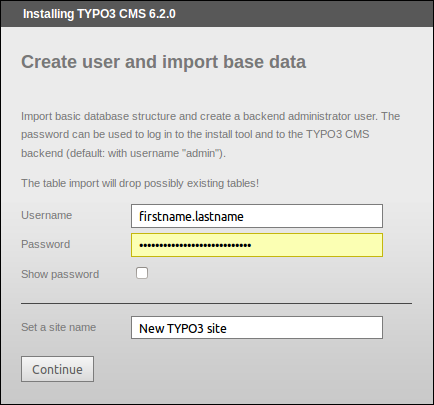
\includegraphics[width=0.8\linewidth]{Images/InstallTool/AdminPasswordAndSiteName.png}
			\end{figure}
		\end{column}

	\end{columns}

\end{frame}

% ------------------------------------------------------------------------------
% Delete All Cache
% ------------------------------------------------------------------------------

\begin{frame}[fragile]
	\frametitle{Strumento di installazione}
	\framesubtitle{Cancellazione di tutte le Cache}

	\begin{itemize}
		\item La nuova funzione in "Azioni importanti" permette agli utenti di cancellare tutte le cache
		\item Essa funziona anche se le cache contengono codice PHP non valido\newline
			(che potrebbe bloccare TYPO3 CMS)
		\item Aggira una istanza di TYPO3 non funzionante, collegandosi direttamente allo Strumento di installazione: \texttt{http://example.com/typo3/install}
	\end{itemize}

	\begin{columns}[T]
		\begin{column}{.3\textwidth}
			\begin{figure}\vspace*{-0.4cm}
				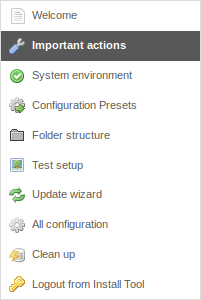
\includegraphics[width=0.7\linewidth]{Images/InstallTool/ImportantActions.png}
			\end{figure}
		\end{column}
		\begin{column}{.7\textwidth}
			\begin{figure}\vspace*{-0.4cm}
				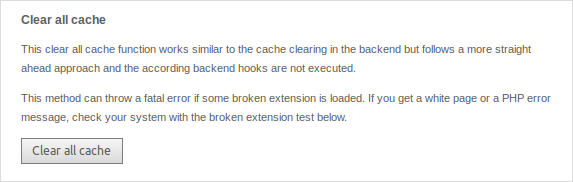
\includegraphics[width=0.9\linewidth]{Images/InstallTool/ClearAllCache.png}
			\end{figure}
		\end{column}
	\end{columns}

\end{frame}

% ------------------------------------------------------------------------------
% Delete All Cache
% ------------------------------------------------------------------------------

\begin{frame}[fragile]
        \frametitle{Strumento di installazione}
        \framesubtitle{Cancellazione di tutte le Cache}

	Sequenza di azioni quando si esegue la "Cancellazione di tutte le cache":

	\begin{enumerate}
		\item Il contenuto della directory \texttt{typo3temp/Cache} è cancellato
		\item Le tabelle del database \texttt{cf\_*} sono svuotate
		\item I files \texttt{ext\_localconf.php} e \texttt{ext\_tables.php}\newline
			sono caricati dalle estensioni
		\item \texttt{flushCaches()} è eseguita
	\end{enumerate}

\end{frame}

% ------------------------------------------------------------------------------
% Check For Broken Extensions
% ------------------------------------------------------------------------------

\begin{frame}[fragile]
	\frametitle{Strumento di installazione}
	\framesubtitle{Verifica di estensioni malfunzionanti}

	\begin{itemize}
		\item La nuova funzionalità in "Azioni importanti" permette agli utenti di verificare,
			se le estensioni possono essere caricate senza malfunzionamenti nel sistema
		\item Molto utile nel passaggio dalla versione TYPO3 4.5 alla 6.2
	\end{itemize}

	\begin{columns}[T]
		\begin{column}{.3\textwidth}
			\begin{figure}\vspace*{-0.4cm}
				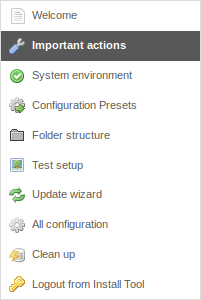
\includegraphics[width=0.7\linewidth]{Images/InstallTool/ImportantActions.png}
			\end{figure}
		\end{column}
		\begin{column}{.7\textwidth}
			\begin{figure}\vspace*{-0.4cm}
				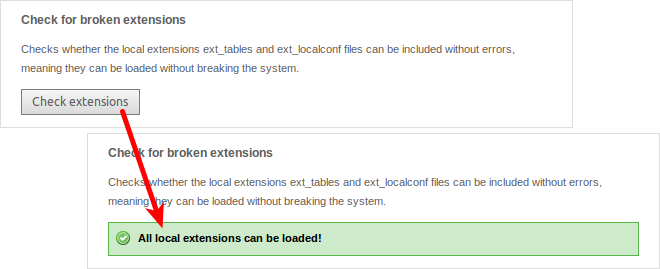
\includegraphics[width=1\linewidth]{Images/InstallTool/CheckForBrokenExtensions.png}
			\end{figure}
		\end{column}
	\end{columns}

\end{frame}

% ------------------------------------------------------------------------------
% Increased Security: Salted Passwords
% ------------------------------------------------------------------------------

\begin{frame}[fragile]
	\frametitle{Strumento di installazione}
	\framesubtitle{Salted Passwords}

	\begin{itemize}
		\item Quando si crea un nuovo utente amministratore di backend con lo\newline 
			Strumento di installazione, è utilizzata una \textbf{salted} password\newline
			(richiede l'installazione, caricamento e configurazione di EXT:saltedpasswords)
		\item La password creata dallo Strumento di installazione è una \textbf{salted}\newline password al meglio
			(al primo login è convertita automaticamente in un hash di tipo MD5)
	\end{itemize}

	\begin{columns}[T]
		\begin{column}{.3\textwidth}
			\begin{figure}\vspace*{-0.4cm}
				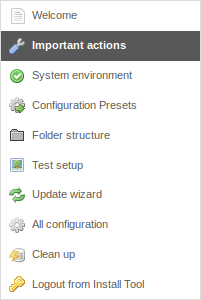
\includegraphics[width=0.7\linewidth]{Images/InstallTool/ImportantActions.png}
			\end{figure}
		\end{column}
		\begin{column}{.7\textwidth}
			\begin{figure}\vspace*{-0.4cm}
				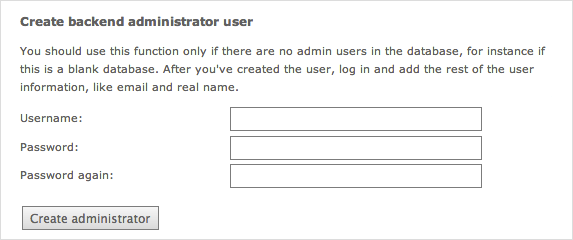
\includegraphics[width=0.9\linewidth]{Images/InstallTool/SaltedPasswords.png}
			\end{figure}
		\end{column}
	\end{columns}

\end{frame}

% ------------------------------------------------------------------------------
% Application Context
% ------------------------------------------------------------------------------

\begin{frame}[fragile]
	\frametitle{Strumento di installazione}
	\framesubtitle{Contesto applicativo (1)}

	\begin{itemize}
		\item TYPO3 >= 6.2 utilizza il \textbf{Contesto applicativo} nei progetti\newline
			\smaller(usato anche in TYPO3 Flow)\normalsize
		\item La variabile di ambiente \texttt{TYPO3\_CONTEXT} imposta il sistema\newline
			\smaller(default: \texttt{Production}, è possibile gestire sottocontesti come \texttt{Production/Staging})\normalsize

			\begin{lstlisting}
				# File: .htaccess
				# Rules to set Application Context based on hostname:

				RewriteCond %{HTTP_HOST} ^dev\.example\.com$
				RewriteRule (.*) $1 [E=TYPO3_CONTEXT:Development]

				RewriteCond %{HTTP_HOST} ^www\.example\.com$
				RewriteRule (.*) $1 [E=TYPO3_CONTEXT:Production]

				# Sets an environment variable, which is then available to TYPO3 CMS:
				SetEnv TYPO3_CONTEXT Production
			\end{lstlisting}

	\end{itemize}

\end{frame}

% ------------------------------------------------------------------------------
% Application Context
% ------------------------------------------------------------------------------

\begin{frame}[fragile]
	\frametitle{Strumento di installazione}
	\framesubtitle{Impostazioni predefinite di TYPO3\_CONF\_VAR}

	\begin{columns}[T]
		\begin{column}{.5\textwidth}

			\begin{itemize}
				\item Alcune impostazioni di \texttt{TYPO3\_CONF\_VAR} possono essere configurate dallo Strumento di installazione
				\item Imposta i controlli come ad esempio debug dell'output, deprecation log, devIPmask e altri log di sistemi e livelli di log
				\item Possibile lavorare in contesti: "Production" e "Development"\newline
					(sono possibili anche configurazioni personalizzate)
			\end{itemize}

		\end{column}
		\begin{column}{.5\textwidth}

			\begin{figure}\vspace*{-0.4cm}
				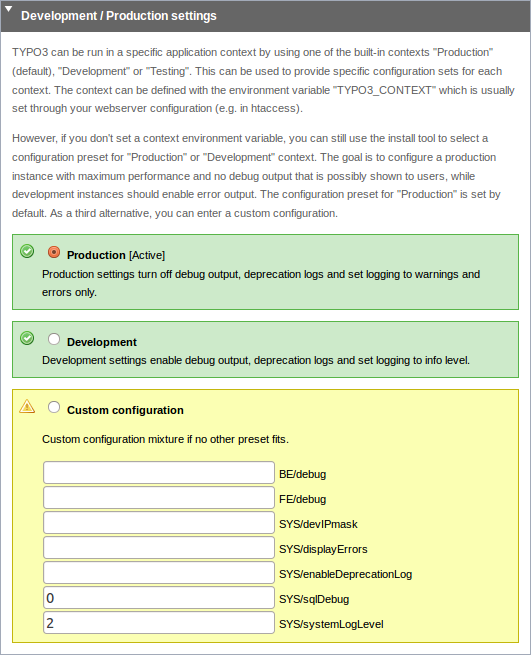
\includegraphics[width=0.8\linewidth]{Images/InstallTool/ApplicationContext.png}
			\end{figure}

		\end{column}
	\end{columns}

\end{frame}

% ------------------------------------------------------------------------------
% Improved Usability
% ------------------------------------------------------------------------------

\begin{frame}[fragile]
	\frametitle{Strumento di installazione}
	\framesubtitle{Usabilità migliorata}

	\begin{columns}[T]
		\begin{column}{.5\textwidth}

			\begin{itemize}
				\item Posizione del menù di sinistra fissa quando si scrolla
					\begingroup\color{typo3red}\textbf{(1)}\endgroup
				\item Posizione fissa del bottone "Scrivi configurazione" in basso
					\begingroup\color{typo3red}\textbf{(2)}\endgroup
				\item Le voci in "Tutte le configurazioni" sono raggruppate (la seziona può essere aperta facendo click sul titolo) e ordinate
					\begingroup\color{typo3red}\textbf{(3)}\endgroup
			\end{itemize}

		\end{column}
		\begin{column}{.5\textwidth}

			\begin{figure}\vspace*{-0.4cm}
				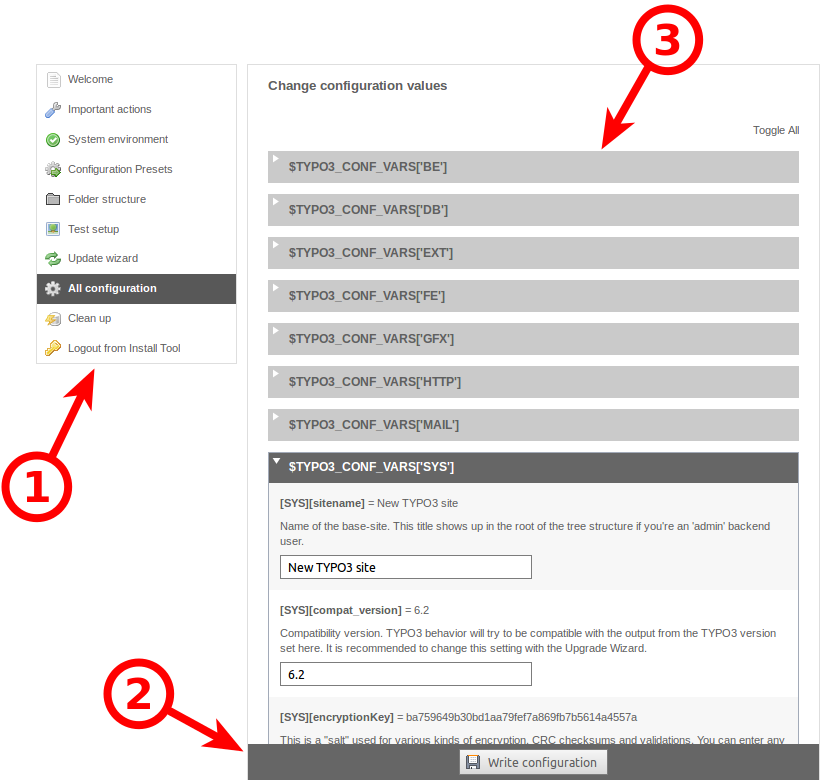
\includegraphics[width=0.8\linewidth]{Images/InstallTool/ImprovedUsability.png}
			\end{figure}

		\end{column}
	\end{columns}

\end{frame}

% ------------------------------------------------------------------------------
% Human-Friendly Error Codes
% ------------------------------------------------------------------------------

\begin{frame}[fragile]
	\frametitle{Strumento di installazione}
	\framesubtitle{Codici di erreore Human-Friendly}

	\begin{itemize}
		\item Sono utilizzate parole chiave significative nei seguenti casi:\newline
			(TYPO3 < 6.2: solo valori numerici)
	\end{itemize}

	\begin{columns}[T]
		\begin{column}{.5\textwidth}
			\advance\leftskip+0.8cm

			\smaller
				\texttt{[SYS][errorHandlerErrors]}\newline
				\texttt{[SYS][exceptionalErrors]}\newline
				\texttt{[SYS][syslogErrorReporting]}\newline
				\texttt{[SYS][belogErrorReporting]}\newline
			\normalsize

		\end{column}
		\begin{column}{.5\textwidth}

			\begin{figure}\vspace*{-0.4cm}
				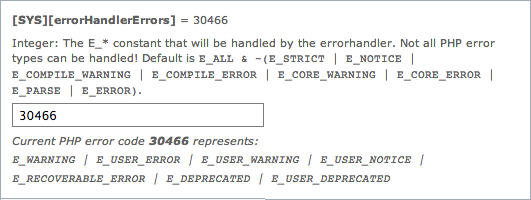
\includegraphics[width=0.9\linewidth]{Images/InstallTool/HumanFriendlyErrorCodes.png}
			\end{figure}

		\end{column}
	\end{columns}

	\begin{itemize}
		\item Un ViewHelper di Extbase \textbf{format.phpErrorCode} si occupa della conversione dei codici di errore di PHP
	\end{itemize}

\end{frame}

% ------------------------------------------------------------------------------
% Errors In Folder Structure
% ------------------------------------------------------------------------------

\begin{frame}[fragile]
	\frametitle{Strumento di installazione}
	\framesubtitle{Errori nella struttura delle directory}

	\begin{itemize}
		\item Errori nella "struttura delle directory" sono visualizzati come badge (numeri cerchiati)
	\end{itemize}

	\begin{figure}
		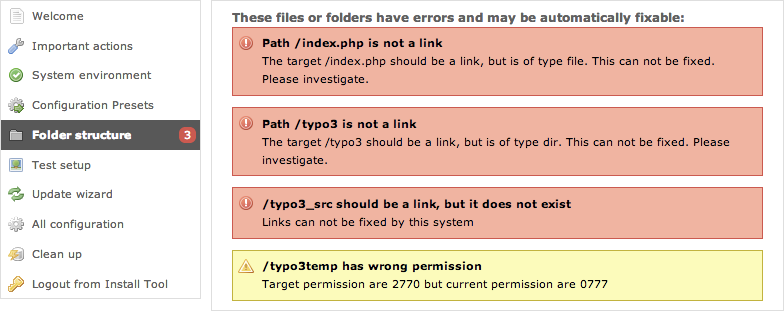
\includegraphics[width=0.95\linewidth]{Images/InstallTool/ErrorsInFolderStructure.png}
	\end{figure}

\end{frame}

% ------------------------------------------------------------------------------
% Core Updates
% ------------------------------------------------------------------------------

\begin{frame}[fragile]
	\frametitle{Strumento di installazione}
	\framesubtitle{Aggiornamenti del core}

	\begin{itemize}
		\item Aggiornamenti del core di TYPO3 all'ultima versione minore con un click su un bottone 
		\item La variabile di sistema \texttt{TYPO3\_DISABLE\_CORE\_UPDATER=1} disabilita questa funzione
	\end{itemize}

	\begin{figure}
		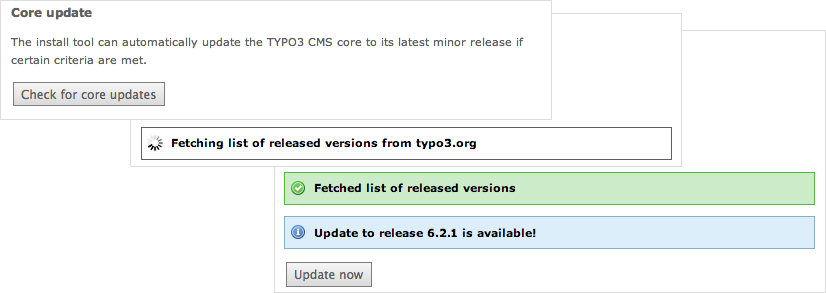
\includegraphics[width=0.95\linewidth]{Images/InstallTool/CoreUpdate.png}
	\end{figure}

\end{frame}

% ------------------------------------------------------------------------------
% Miscellaneous
% ------------------------------------------------------------------------------

\begin{frame}[fragile]
	\frametitle{Strumento di installazione}
	\framesubtitle{Varie}

	\begin{itemize}
		\item Tutti i form sono protetti con CSRF (\textit{cross-site request forgery})
		\item Lo strumento di installazione utilizza un Fluid Standalone View semplificato
		\item Solo le funzioni essenziali di TYPO3 sono caricate\newline
			(problemi in \texttt{ext\_localconf.php} o \texttt{ext\_tables.php} di un estensione non blocca più lo strumento di installazione)
		\item Nuovo punto di partenza:	\tabto{3.2cm} \texttt{typo3/sysext/install/Start/Install.php}\newline
			Prima:					\tabto{3.2cm} \texttt{typo3/install/index.php}\newline
									\tabto{3.2cm} (redirezione dal vecchio al nuovo URL)
		\item La disattivazione della cache permette allo strumento di installazione di funzionare, anche se la cache contiene codice PHP non valido
	\end{itemize}

\end{frame}

% ------------------------------------------------------------------------------
% Miscellaneous
% ------------------------------------------------------------------------------

\begin{frame}[fragile]
	\frametitle{Strumento di installazione}
	\framesubtitle{Varie}

	\begin{itemize}
		\item Verifica se l'opzione PHP \texttt{xdebug.max\_nesting\_level} mostra un valore di 250 o più (il valore di default "100" potrebbe creare problemi)
		\item "Verifica dei permessi":

			\small
				Se la directory web principale non ha i permessi corretti (es. "2770"),
				e questo problema non è risolto, es. perchè la directory non appartiene
				all'utente di sistema che usa lo strumento di installazione, il primo passo
				dell'installazione si blocca.
				L'opzione "targetPermissionRelaxed" abbassa i controlli se i permessi non 
				sono corretti, permettendo la continuazione dell'installazione fino a quando
				non è necessario creare sottodirectory.
			\normalsize

	\end{itemize}

\end{frame}

% ------------------------------------------------------------------------------
% Miscellaneous
% ------------------------------------------------------------------------------

\begin{frame}[fragile]
	\frametitle{Strumento di installazione}
	\framesubtitle{Varie}

	\begin{itemize}
		\item Rimosse le seguenti opzioni (chiavi) dallo strumento di installazione\newline
			(e di conseguenza anche dal file \texttt{LocalConfiguration.php}):
	\end{itemize}

	\begin{columns}[T]
		\begin{column}{.5\textwidth}
			\advance\leftskip+0.8cm
			\smaller
				\texttt{BE/loginLabels}\newline
				\texttt{BE/loginNews}\newline
				\texttt{BE/useOnContextMenuHandler}\newline
				\texttt{EXT/em\_mirrorListURL}\newline
				\texttt{EXT/em\_wsdlURL}\newline
				\texttt{EXT/extList}\newline
				\texttt{EXT/extList\_FE}\newline
				\texttt{EXT/noEdit}\newline
			\normalsize
		\end{column}
		\begin{column}{.5\textwidth}
			\smaller
				\texttt{FE/defaultTypoScript\_editorcfg}\newline
				\texttt{FE/simulateStaticDocuments}\newline
				\texttt{GFX/noIconProc}\newline
				\texttt{GFX/TTFLocaleConv}\newline
				\texttt{SYS/additionalAllowedClassPrefixes}\newline
				\texttt{SYS/caching/cacheBackends}\newline
				\texttt{SYS/caching/cacheFrontends}\newline
				\texttt{SYS/extCache}\newline
				\texttt{SYS/T3instID}\newline
			\normalsize
		\end{column}

	\end{columns}

\end{frame}

% ------------------------------------------------------------------------------

